
\section{Metodología}
\label{sec:metodologia}

En el diseño típico de un sistema de punto fijo se emplea el  flujo observado en la Figura \ref{fig:fig2}. Si bien el sistema ya se encuentra implementado, corresponderá al proyecto actual implementarlo en el SoC PolarFire MPFS095T, corriendo las diferentes pruebas ofrecidas por el diseñador del sistema para verificarlo a nivel comportamental y funcional. Cabe destacar que este algoritmo está totalmente implementado en hardware. 


\begin{figure}[ht]
  \centering
  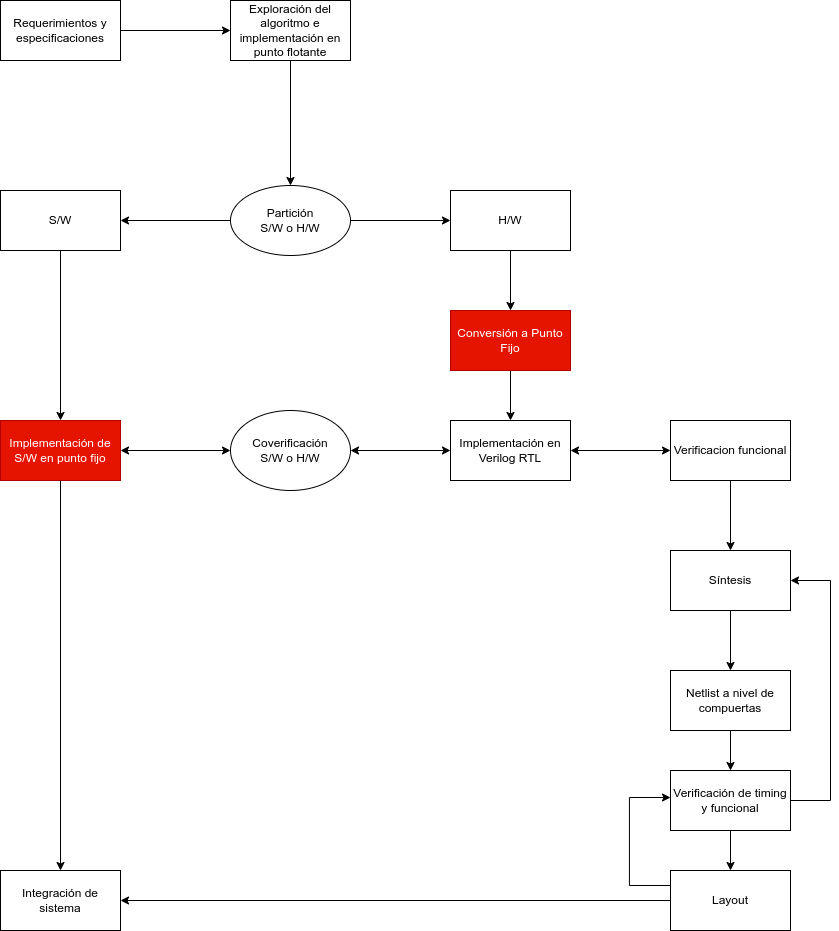
\includegraphics[width=0.8\textwidth]{figures/2.png}
  \caption{\label{fig:fig2}Flujo típico de diseño de sistema en punto fijo}
\end{figure}
Para la implementación del firmware se utiliza la metodología TDD (\textit{Test Driven Development}), que como lo indican sus siglas se basa en el desarrollo guiado por pruebas, y se encuentra ampliamente difundido en la actualidad en el mundo del software embebido. En la Figura \ref{fig:fig3} observamos el ciclo de desarrollo típico de esta metodología. Son numerosas las ventajas de esta decisión de diseño, pero la principal es que al ser el primordial objetivo conseguir un firmware de nivel industrial que se destaque por su robustez y flexibilidad, es esencial conseguir un nivel de \textit{coverage} del 100\%.

\begin{figure}[ht]
  \centering
  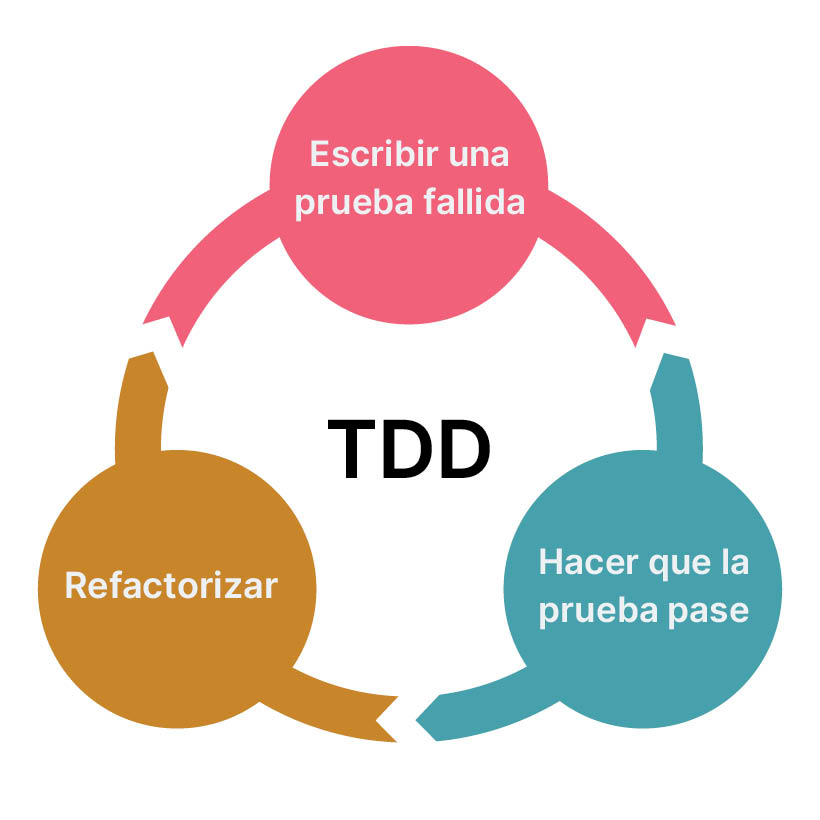
\includegraphics[width=1\textwidth]{figures/3.jpg}
  \caption{\label{fig:fig3}Desarrollo guiado por pruebas}
\end{figure}


 El framework de TDD elegido para desarrollar el código es \textit{Ceedling}, pensado para desarrollar firmware para embebidos en ANSI C, lo cual es parte del proyecto. Para la administración del proyecto se hará uso de la herramienta \textit{Org Mode + Projectile}, que permitirá controlar el cumplimiento de los plazos establecidos en la Planificación (Ver Sección \ref{sec:etapas} ).
\par Por ultimo recalcar que para la programación de la placa de desarrollo, es decir del FPGA se hará uso del software provisto por el fabricante Libero\textregistered, y para la programación del sistema de microprocesadores se hará uso de otro software del fabricante llamado Softconsole\textregistered.
%%% Local Variables:
%%% mode: LaTeX
%%% TeX-master: "../anteproyecto"
%%% End:
